\section{Experimental Details \& Further Discussion}\label{sec:appendix_experimental_details}

\subsection{Relational Games (\Cref{ssec:relgames})}\label{ssec:appendxi_relgames}

\subsubsection*{Experimental details}

\textbf{Dataset details.} The relational games benchmark datasets consists of $36 \times 36 \times 3$ RGB images depicting a $3 \times 3$ grid of objects which satisfy a particular visual relationship. The set of objects consists of simple geometric shapes. For example, in the \texttt{occurs} task, one object is present in the top row and three in the bottom row, and the task is to determine whether the object in the top row occurs (i.e., is among) the objects in the bottom row. The most difficult task in the benchmark is the \texttt{match pattern} task, where the grid contains a triplet of objects in the top row and another triplet of objects in the bottom row. Each triplet satisfies some relationship (e.g., ABC, ABA, ABB, or AAB), and the task is determine whether the relation in the first triplet is the same as the relation in the second triplet. The difficulty in solving this task is that it requires parsing a second-order relation (a relation between relations). We remark that composing relational attention modules naturally captures this kind of hierarchical relations: one relational attention operation produces objects with a relational representation and another would compute relations between those relations.

\aanote{TODO -- add figure depicting relational games tasks?}

\textbf{Model architectures.} We use a Vision-Transformer-type architecture where the input image is split up into patches, flattened, and passed through the sequence model with added learned positional embeddings. We use average pooling at the end and pass through an MLP to produce the final prediction. We use a patch size of $12 \times 12$ which separates objects according to the grid structure. We note that in more general visual relational reasoning tasks where there isn't this type of grid structure, it would be appropriate to combine our approach with an object-discovery module such as Slot Attention~\citep{locatelloObjectCentricLearningSlot2020}.

We use the following hyperparameters: 2 layers, $\dmodel = 128$, $\dff = 256$, SwiGLU ``activation'', dropout rate = 0.1, and pre-LayerNormalization. For the Orthrus models, we use positional symbols as the symbol assignment mechanism. The total number of heads is 2. For the Transformer model, there are only self-attention heads: $\nhsa = 2$. For Orthrus, we evaluated two configurations for the composition of head types, one with $\nhsa = \nhra = 1$ and one with only relational attention heads $\nhsa = 0, \nhra = 2$. We also evaluated variants with and without the constraint that the relations in relational attention are symmetric (i.e., $\Wqrel = \Wkrel$).

\textbf{Training details.} For each task and model, we evaluated learning curves by varying the training set size and training the model until convergence, then evaluating on a hold-out test sets. For four out of five of the tasks, we evaluate learning curves within the range of $250$ to $2,500$ samples, in increments of $250$. For the more difficult \texttt{match pattern}, the range is from $5,000$ to $25,000$ in increments of $5,000$. The ranges were chosen based on the difficulty of the different tasks in order to identify the right ``resolution''. When evaluating learnign curves, each training set is sampled random from the full dataset. For each task, model, and training set size, we repeat the experiment 5 times with different random seeds to compute approximate confidence intervals (accounting for randomness in sampling the dataset and random initialization). We use an Adam optimizer with a learning rate of $0.001$, $\beta_1 = 0.9, \beta_2 = 0.99$, and a batch size of $512$. We train for 50 epochs.

\subsubsection*{Further Discussion, Exploration, \& Ablations}

We performed an ablation over the \textit{symmetry} inductive bias in the relations computed in relational attention. Our implementation exposes an argument which controls whether the relation $r(x, y) = (\iiprod{\Wqrell{\ell}}{\Wkrell{\ell}})_{\ell \in [d_r]} \in \reals^{d_r}$ modeled in relational attention is constrained to be symmetric by setting $\Wqrell{\ell} = \Wkrell{\ell}$. Indeed, we find symmetry to be a useful inductive bias in this task.~\Cref{fig:relgames_symmetry_ablation} depicts learning curves for the two configurations of Orthrus comparing symmetric RA against asymmetric RA. We find that symmetry results in faster learning curves for both configurations.

\begin{figure}[h]
    \centering
    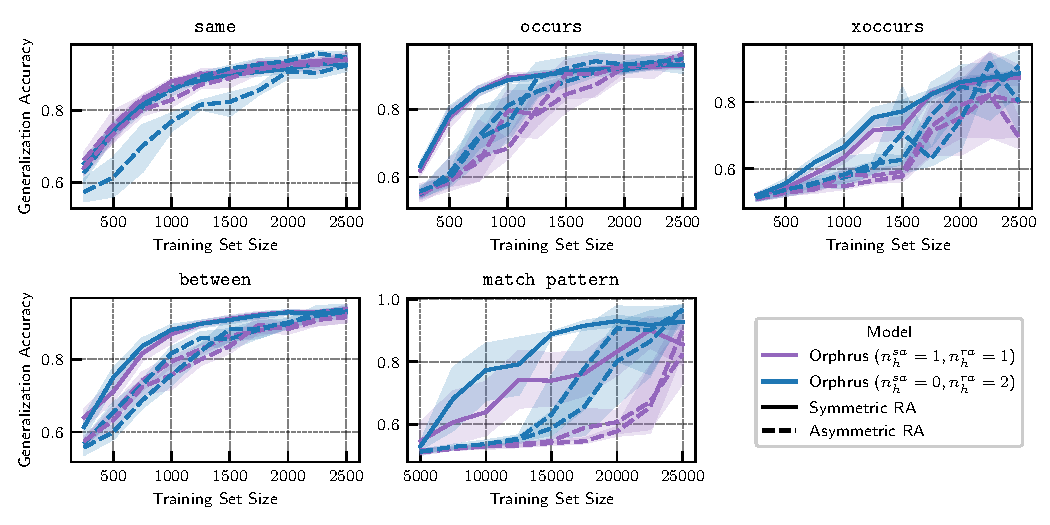
\includegraphics[width=\textwidth]{figs/experiments/relgames/relgames_learning_curves_symmetry_ablation.pdf}
    \caption{An ablation of the effect of symmetry in relational attention in the relational games experiments.}\label{fig:relgames_symmetry_ablation}
\end{figure}

\subsection{Mathematical Problem-Solving (\Cref{ssec:math})}\label{ssec:appendix_math}

\subsubsection*{Experimental details}

\textbf{Dataset details.} \citet{saxtonAnalyzingMathematicalReasoning2019} propose a benchmark to assess neural models' ability to perform mathematical reasoning. The dataset consists of a suite of tasks in free-form textual input/output format. The tasks cover several topics in mathematics, including arithmetic, algebra, and calculus. For each task, the authors programmatically generate $2 \times 10^6$ training examples and $10^4$ validation examples. Questions have a maximum length of 160 characters and answers have a maximum length of 30 characters.

\aanote{TODO -- add examples of input-output sequences for tested tasks?}

\textbf{Model architectures.} We use an an encoder-decoder architecture for this experiment, treating it as a sequence-to-sequence task. We use character-level encoding with a common alphabet of size 85 containing small and upper case letters, digits 0-9, and symbols (e.g., \texttt{*, /, +, -}). The models have 2-layer encoders and decoders, with $\dmodel = 128, \dff = 256$, ReLU activation, dropout rate = 0.1, and post-normalization. Sinusoidal positional embeddings are used as the positional encoding method. For all models the total number of attention heads (across self-attention and relational attention) is $8$. For the Transformer model, there are only self-attention heads: $\nhsa = 8$ for both the encoder and decoder. For Orthrus, we evaluated two configurations for the composition of head types, one with $\nhsa = \nhra = 4$ in the encoder and $\nhsa = 8, \nhra = 0$ in the decoder (i.e., standard Transformer Decoder), and one with $\nhsa = 4 = \nhra = 4$ in the encoder and $\nhsa = 4 = \nhra = 4$ in the decoder. The number of cross-attention heads in the decoder is $8$ in all cases. No symmetry constraint is made on relational attention. Position-relative symbols are used as the symbol assignment mechanism, and are shared across all layers in both the encoder and decoder.

\textbf{Training Details.} Each model is trained on each task for 50 epochs. We use the Adam optimizer with $\beta_1 = 0.9, \beta_2 = 0.995$, a learning rate of $6 \times 10^{-4}$, and a batch size of 128. We evaluate and track the per-character accuracy over the course of training. We repeat this process 5 times for each combination of model and task with different random seeds to compute approximate confidence intervals.

\subsubsection*{Further Discussion, Exploration, \& Ablations}

This benchmark contains two validation splits: an interpolation split and an extrapolation split. The interpolation split is generated by the same procedure as the training split. The extrapolation split is generated with different parameters to make the task more difficult. We refer to the original reference for more details~\citep{saxtonAnalyzingMathematicalReasoning2019}.~\Cref{fig:math_training_curves_interpolation} in the main text depicts the interpolation validation accuracy.~\Cref{fig:math_training_curves_extrapolation} depicts the extrapolation validation accuracy over the course of training. For completeness, we also show the training accuracy in~\Cref{fig:math_training_curves_trainacc}.

\begin{figure}
    \centering
    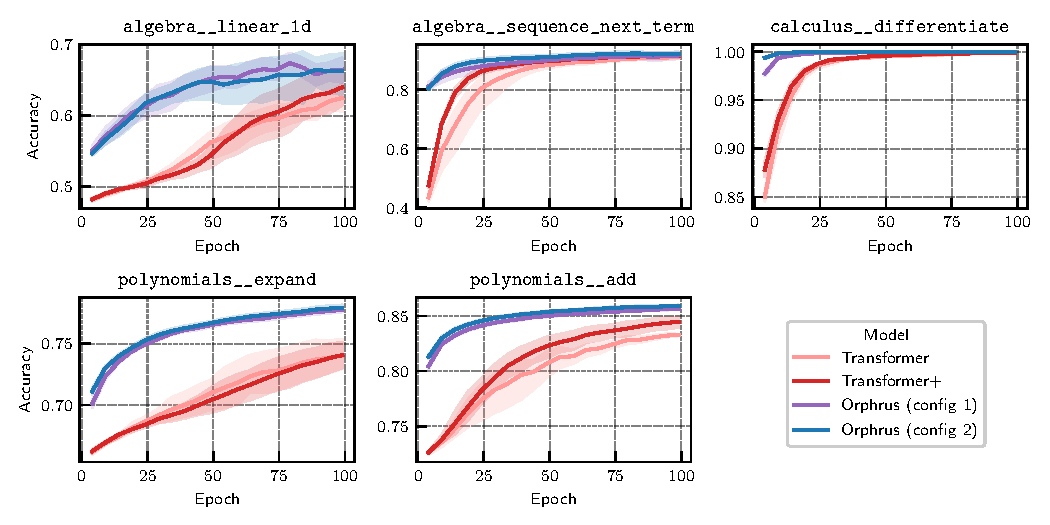
\includegraphics[width=\textwidth]{figs/experiments/math/math_training_curves_extrapolation.pdf}
    \caption{Extrapolation validation accuracy over the course of training for mathematical problem-solving tasks.}\label{fig:math_training_curves_extrapolation}
\end{figure}

\begin{figure}
    \centering
    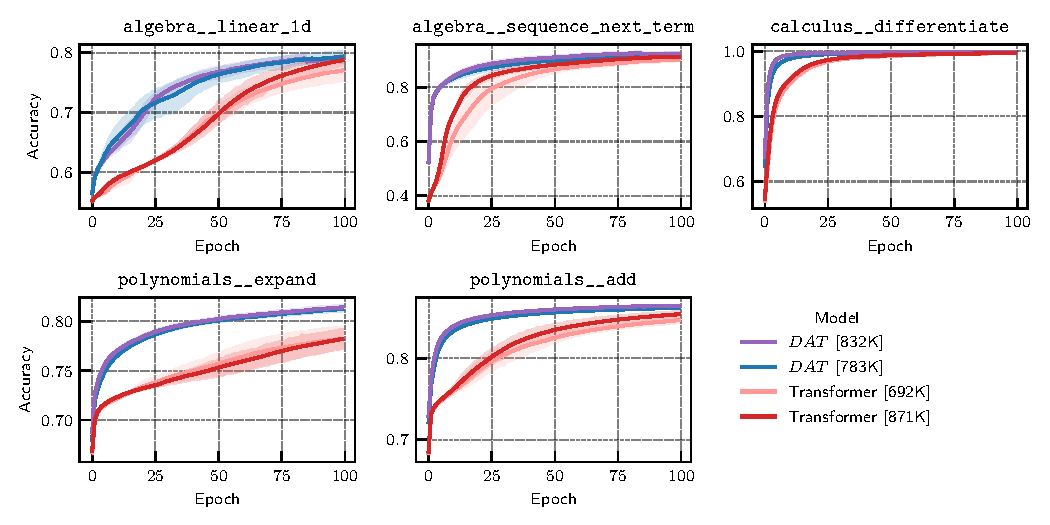
\includegraphics[width=\textwidth]{figs/experiments/math/math_training_curves_trainacc.pdf}
    \caption{Training accuracy over the course of training for mathematical problem-solving tasks.}\label{fig:math_training_curves_trainacc}
\end{figure}


\subsection{Language Modeling (\Cref{ssec:tiny_stories})}\label{ssec:appendix_lm}

\subsubsection*{Experimental details}

\aanote{TODO -- add samples of generated input? compare across models. add samples of stories from dataset?}

\textbf{Dataset details.} The Tiny Stories dataset by~\citet{eldanTinyStoriesHowSmall2023} is a language modeling benchmark designed to evaluate small language models. The dataset consists of short stories and is synthetically generated by GPT-3.5 and GPT-4.

\textbf{Model architectures.} We use an Decoder-only architecture (can also be seen as an encoder-only architecture), with causal attention for autoregressive language modeling. We fix the total number of attention heads to be $8$ for all models. For the Transformer model, there are only self-attention heads: $\nhsa = 2$. For Orthrus, we evaluated two configurations for the composition of head types, one with $\nhsa = 6, \nhra = 2$ (more self-attention heads) and one with $\nhsa = \nhra = 4$ (a balanced composition of head types). We experiment with $\dmodel \in \sset{64, 128}$ and number of layers $L \in \sset{4, 5, 6}$. For all models, we use $\dff = 4 \dmodel$, SwiGLU activation in the MLP, RoPE positional encoding, no bias, dropout rate = 0.1, and pre-LayerNormalization. We use weight-tying between the embedding layer and the final prediction layer~\citep{inanTyingWordVectors2016}. For Orthrus models, we perform ablations on the effect of the choice of symbol assignment mechanism and symmetry in relational attention. We train models with position-relative symbols and symbolic attention, as well as models with symmetric and asymmetric relations in relational attention. We use a context size of 512 for all models. Text is tokenized using the Llama SentencePiece tokenizer~\citep{touvronLlamaOpenFoundation2023}, which contains $32,000$ tokens.

\Cref{fig:tiny_stories_val_loss_curves} in the main text depicts the $\dmodel = 64$ models with varying number of layers $L \in \sset{4, 5, 6}$.~\Cref{fig:tiny_stories_val_loss_curves_d128} shows the loss curves for larger models with $\dmodel = 128$. The Orthrus models use symbolic attention as the symbol assignment mechanism and asymmetric relations in relational attention. Symbolic attention uses $n_s = \texttt{context\_length} = 512$ symbols with 4 heads.

\textbf{Training Details.} All models are trained with the AdamW optimizer with a constant learning rate of $0.001$ and $\beta_1 = 0.9, \beta_2 = 0.95$. We clip gradients to a norm of 1. Models are trained for $100,000$ iterations. We use a batch size of $128$ with $2$ gradient accumulation steps. Thus, each step trains on $131,072$ tokens.

\begin{table}
    \caption{Language Modeling on the Tiny Stories Dataset}\label{tab:tiny_stories_results}
    
\begin{tabular}{@{}|c|c|c|c|c|c|c|c|@{}}
\toprule
$\dmodel$             & $L$                & $\nhsa$            & $\nhra$            & Symbol Assignment Mechanism                & Symmetric RA & val/loss       & val/perplexity \\
\midrule
\multirow{23}{*}{64}  & \multirow{9}{*}{4} & \multirow{4}{*}{4} & \multirow{4}{*}{4} & \multirow{2}{*}{Position-Relative Symbols} & False        & 1.764          & 5.840          \\
                        &                    &                    &                    &                                            & True         & 1.785          & 5.963          \\ \cline{5-8} 
                        &                    &                    &                    & \multirow{2}{*}{Symbolic Attention}        & False        & \textbf{1.729} & \textbf{5.639} \\
                        &                    &                    &                    &                                            & True         & 1.744          & 5.722          \\ \cline{3-8} 
                        &                    & \multirow{4}{*}{6} & \multirow{4}{*}{2} & \multirow{2}{*}{Position-Relative Symbols} & False        & 1.768          & 5.859          \\
                        &                    &                    &                    &                                            & True         & 1.777          & 5.914          \\ \cline{5-8} 
                        &                    &                    &                    & \multirow{2}{*}{Symbolic Attention}        & False        & 1.740          & 5.697          \\
                        &                    &                    &                    &                                            & True         & 1.745          & 5.727          \\ \cline{3-8} 
                        &                    & 8                  & 0                  & NA                                         & NA           & 1.775          & 5.903          \\ \cline{2-8} 
                        & \multirow{6}{*}{5} & \multirow{2}{*}{4} & \multirow{2}{*}{4} & \multirow{2}{*}{Symbolic Attention}        & False        & \textbf{1.692} & \textbf{5.431} \\
                        &                    &                    &                    &                                            & True         & 1.698          & 5.467          \\ \cline{3-8} 
                        &                    & \multirow{3}{*}{6} & \multirow{3}{*}{2} & Position-Relative Symbols                  & True         & 1.730          & 5.640          \\ \cline{5-8} 
                        &                    &                    &                    & \multirow{2}{*}{Symbolic Attention}        & False        & \textbf{1.692} & \textbf{5.432} \\
                        &                    &                    &                    &                                            & True         & 1.704          & 5.495          \\ \cline{3-8} 
                        &                    & 8                  & 0                  & NA                                         & NA           & 1.730          & 5.640          \\ \cline{2-8} 
                        & \multirow{8}{*}{6} & \multirow{4}{*}{4} & \multirow{4}{*}{4} & \multirow{2}{*}{Position-Relative Symbols} & False        & 1.685          & 5.395          \\
                        &                    &                    &                    &                                            & True         & 1.704          & 5.498          \\ \cline{5-8} 
                        &                    &                    &                    & \multirow{2}{*}{Symbolic Attention}        & False        & \textbf{1.656} & \textbf{5.239} \\
                        &                    &                    &                    &                                            & True         & 1.668          & 5.303          \\ \cline{3-8} 
                        &                    & \multirow{3}{*}{6} & \multirow{3}{*}{2} & Position-Relative Symbols                  & True         & 1.691          & 5.424          \\ \cline{5-8} 
                        &                    &                    &                    & \multirow{2}{*}{Symbolic Attention}        & False        & 1.663          & 5.277          \\
                        &                    &                    &                    &                                            & True         & 1.669          & 5.308          \\ \cline{3-8} 
                        &                    & 8                  & 0                  & NA                                         & NA           & 1.692          & 5.431          \\ \hline
\multirow{10}{*}{128}   & \multirow{5}{*}{4} & \multirow{2}{*}{4} & \multirow{2}{*}{4} & \multirow{2}{*}{Symbolic Attention}        & False        & \textbf{1.411} & \textbf{4.102} \\
                        &                    &                    &                    &                                            & True         & 1.417          & 4.127          \\ \cline{3-8} 
                        &                    & \multirow{2}{*}{6} & \multirow{2}{*}{2} & \multirow{2}{*}{Symbolic Attention}        & False        & 1.412          & 4.105          \\
                        &                    &                    &                    &                                            & True         & 1.415          & 4.118          \\ \cline{3-8} 
                        &                    & 8                  & 0                  & NA                                         & NA           & 1.431          & 4.183          \\ \cline{2-8} 
                        & \multirow{5}{*}{6} & \multirow{2}{*}{4} & \multirow{2}{*}{4} & \multirow{2}{*}{Symbolic Attention}        & False        & \textbf{1.337} & \textbf{3.811} \\
                        &                    &                    &                    &                                            & True         & 1.346          & 3.843          \\ \cline{3-8} 
                        &                    & \multirow{2}{*}{6} & \multirow{2}{*}{2} & \multirow{2}{*}{Symbolic Attention}        & False        & 1.340          & \textbf{3.818} \\
                        &                    &                    &                    &                                            & True         & 1.346          & 3.843          \\ \cline{3-8} 
                        &                    & 8                  & 0                  & NA                                         & NA           & 1.353          & 3.870          \\ \bottomrule
\end{tabular}%
\end{table}
\aawarning{TODO -- Table is incomplete; remove table or remove certain cells. or run missing configs}

\begin{figure}
    \centering
    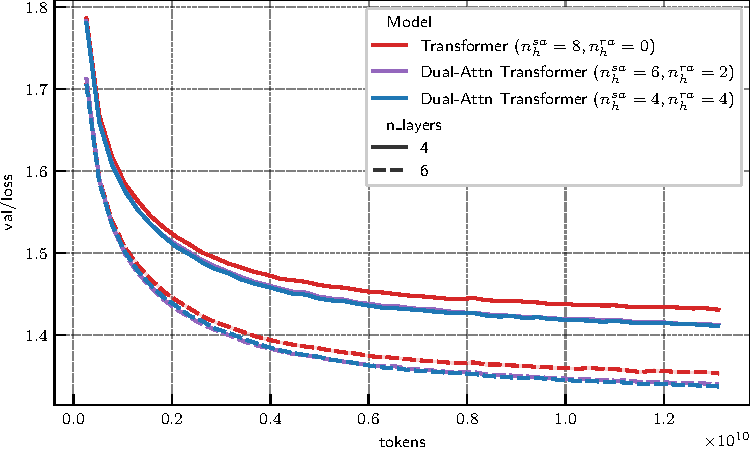
\includegraphics[width=0.5\textwidth]{figs/experiments/tiny_stories/d128L4L6_symattn_asymra.pdf}
    \caption{Loss curves of Orthrus language models with $\dmodel = 128$.}\label{fig:tiny_stories_val_loss_curves_d128}
\end{figure}
\aawarning{$\dmodel = 128$ loss curves are missing $\nhsa=\nhra=4$.}

\subsection*{Further Discussion, Exploration, \& Ablations}

\begin{figure}
    \centering
    \begin{subfigure}[t]{0.45\textwidth}
        \centering
        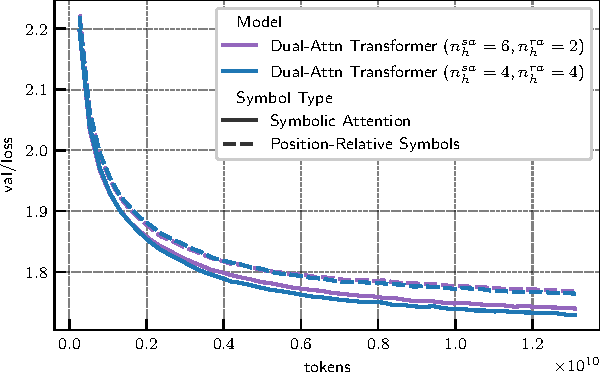
\includegraphics[width=\textwidth]{figs/experiments/tiny_stories/d64L4_ablation_symboltype_asymra.pdf}
        \caption{$d=64, L=4$, asymmetric RA.}
    \end{subfigure}
    \hfill
    \begin{subfigure}[t]{0.45\textwidth}
        \centering
        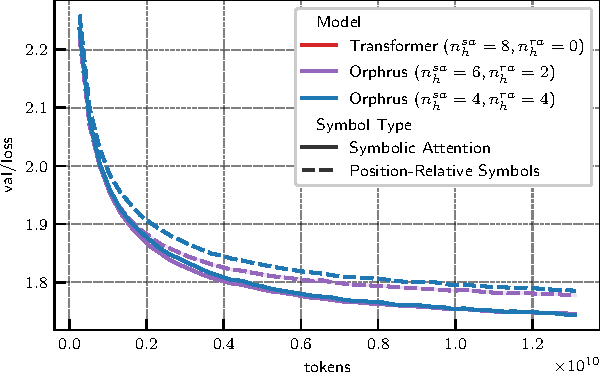
\includegraphics[width=\textwidth]{figs/experiments/tiny_stories/d64L4_ablation_symboltype_symra.pdf}
        \caption{$d=64, L=4$, symmetric RA.}
    \end{subfigure}
    \caption{Ablation of symbol assignment mechanism. Symbolic attention outperforms position-relative symbols.}\label{fig:ablation_symbol_type}
\end{figure}

\begin{figure}
    \centering
    \begin{subfigure}[t]{0.45\textwidth}
        \centering
        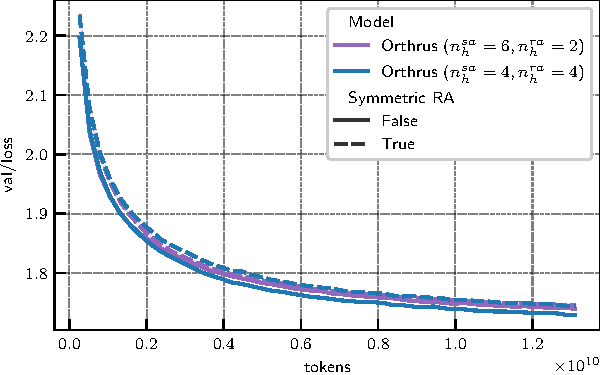
\includegraphics[width=\textwidth]{figs/experiments/tiny_stories/d64L4_ablation_symmetry_symmattn.pdf}
        \caption{$d = 64, L = 4$, symbolic attention.}
    \end{subfigure}
    \hfill
    \begin{subfigure}[t]{0.45\textwidth}
        \centering
        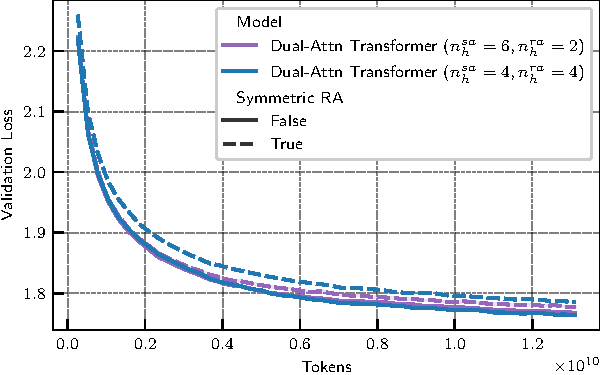
\includegraphics[width=\textwidth]{figs/experiments/tiny_stories/d64L4_ablation_symmetry_posrelsym.pdf}
        \caption{$d = 64, L = 4$, postion-relative symbol assignment}
    \end{subfigure}
    \caption{Ablation of Symmetry in relational attention. The Orthrus models with asymmetric relations perform slightly better than those with a symmetry constraint.}\label{fig:ablation_symmetry}
\end{figure}

\Cref{tab:tiny_stories_results} shows the end-of-training validation loss and perplexity for all models we evaluated. For each $\dmodel, L$ the best-performing model is bolded. We find that the Orthrus model with asymmetric relational attention and symbolic attention consistently performs the best, beating out the Transformer by a small margin.

\Cref{fig:ablation_symbol_type} depicts an ablation over symbol type. For $\dmodel = 64, L = 4$, it shows training curves for Orphrus models with two types of symbol retrieval mechanism: symbolic attention and position-relative symbol. We find that the symbolic attention variant learns faster and reaches smaller loss. This holds both when relational attention uses symmetric or asymmetric relations. We posit the explanation that the differentiable equivalence class mapping implemented by symbolic attention may capture a form of syntax.

\Cref{fig:ablation_symmetry} shows an ablation over symmetry of relational attention. Relational attention can be constrained to represent symmetric relations by imposing that $\Wqrel = \Wkrel$. This is sometimes a useful inductive bias, as observed for the relational games experiments. However, in the language modeling experiments, we found that it was not a useful inductive bias and that asymmetric relational attention outperformed symmetric relational attention. One possible explanation is that the types of relations that are relevant in parsing language are in general asymmetric. For example, syntactic or grammatical relations such as noun-verb, subject-object, determiner-noun, etc. are asymmetric.

\subsection{Image Recognition (\Cref{ssec:imagenet})}

\subsubsection*{Experimental details}

\textbf{Dataset details.} For this experiment, we use the ImageNet Large Scale Visual Recognition Challenge 2012 (ILSVRC2012) dataset~\citep{imagenet}. The dataset is roughly 140GB in size and consists of $224 \times 224$ RGB images hand-labeled with the presence or absence of 1,000 object categories.

\textbf{Model architectures.} We use a Vision Transformer-style architecture \citep{dosovitskiyImageWorth16x162020}. ImageNet's $224 \times 224 \times 3$ RGB images are divided into $16 \times 16$ patches, flattened, and linearly embedded into a vector. A learnable positional embedding is added to each patch embedding. We also prepend a special classification token. The sequence of patch embeddings are then fed through an Encoder and the embedding of the class token is used to generate the final classification through a fully connected layer. We compare a Vision Transformer model with $n_h^{sa} = 16$ to an Orthrus model with $n_h^{sa} = 10, n_h^{sa} = 6$. For both, we used a model dimension $\dmodel = 1024$, $L = 24$ layers, MLP hidden dimension $\dff = 4096$, SwiGLU activation, no bias, dropout rate = 0.1, and pre-LayerNormalization. The Orthrus model uses position-relative symbols as the symbol assignment mechanism and symmetric relational attention.

\textbf{Training details.} Both models are trained with the AdamW optimizer, with a constant learning rate of $5 \times 10^{-4}$ and $\beta_1 = 0.9, \beta_2 = 0.99$. We used a batch size of 32 and 32 gradient accumulation steps.